\documentclass[12pt]{article}
\usepackage[slovene]{babel}
\usepackage[utf8]{inputenc}
\usepackage[T2A]{fontenc}
\usepackage{amsmath}
\usepackage{amsfonts}
\usepackage{amssymb}
\usepackage[version=4]{mhchem}
\usepackage{stmaryrd}
\usepackage{graphicx}
\usepackage[export]{adjustbox}
\graphicspath{ {./images/} }
\usepackage{physics}
\usepackage{geometry}
\geometry{left=2cm,right=2cm,top=2cm,bottom=2cm}

\title{\textbf{Millikanov poskus}}
\author{Samo Krejan}
\date{maj 2025}

\begin{document}
\maketitle

\section{Uvod}

Millikanov poskus je zgodovinsko zelo pomemben, saj je prvi določil vrednost osnovnega naboja $e_0$. To je dosegel tako, da je obravnaval nabite oljne kapljice v zraku pod uplivom električnega polja $E$. Ko kaplica neha pospeševati, nanjo delujejo tri sile, katerih vsota je enaka $0$. Te sile so; gravitacijska sila, sila upora (Stokesova sila) in električna sila. Električno polje lahko kaže v smeri gravitacijskega pospeška $(+)$ ali pa proti njemu $(-).$ Ravnovesje sil se izrazi kot \ref{sile}:

\begin{equation}
    \frac{4\pi r^3}{3} (\rho_0-\rho_z)g \pm n e_0 E = 6\pi r \eta v_\pm
    \label{sile}
\end{equation}
Tu je $\rho_0$ gostota olja, $\rho_z$ gostota zraka, $E = U/d$ jakost električnega polja, $e_0$ osnovni naboj, $n$ število osnovnih nabojev v kapljici in $\eta$ viskoznost zraka. Če za posamezno kaplico izmerimo hitrost v polju, usmerjenem dol in gor, lahko določimo radij kapljice \ref{radi}, ter naboj kapljice \ref{naboj} kot:

\begin{equation}
    r = \sqrt{\frac{9 \eta (v_+ + v_-)}{4g(\rho_0-\rho_z)}}
    \label{radi}
\end{equation}

\begin{equation}
    ne_0 = \frac{3\pi r \eta}{E}(v_+ - v_-)
    \label{naboj}
\end{equation}

\section{Potrebščine}

\begin{itemize}
    \item Millikanov aparat: kondenzator, razpršilec z oljem, LED za osvetljevanje,
    \item mikroskop s kamero, ki je priključena na računalnik,
    \item usmernik za 300V,
    \item preklopnik smeri napetosti,
    \item voltmeter.
\end{itemize}


\section{Naloga}

\begin{enumerate}
    \item Izmeri hitrosti gibanja kapljiv v električnem in gravitacijskem polju,
    \item iz meritve izračunaj hitrost kapljic in njihov naboj, ter določi osnovni naboj.
\end{enumerate}


\section{Rezultati in analiza}

Najprej smo izmerili napetost na kondenzatorju, ki smo ji nato le preklapljali smer. Napetost je bila $250\pm 1\ V$, razmak med elektrodama kondenzatorja pa $5.0\pm 0.1\ mm$ kar nam da električno polje v kondenzatorju $E = 5.0\ pm 1\ V/m$. Za gostoto olja smo uporabili $\rho_0 = 973 kg/m^3$, za gostoto zraka pa $\rho_z = 1.3 kg/m^3$. Viskoznost zraka je $\eta = 1.83 \cdot 10^{-5}\ Pas$. V tabelo smo nato zapisali preračunane vrednosti za $r$ in $ne$, ter nato določili še posamezne vrednosti za $n$ in $e_0$. Glej tabelo \ref{tabela}:

\begin{table}[!ht]
\centering
\begin{tabular}{c|c||c|c|c|c}
v- & v+ & r & ne & $n$ & $e_0$ \\\hline \hline
29.0+/-2.0 & 33.0+/-2.0 & 0.518+/-0.012 & (7+/-5)e-21 & 0 & NaN \\
40.0+/-2.0 & 43.0+/-2.0 & 0.599+/-0.010 & (6+/-6)e-21 & 0 & NaN \\
60.0+/-2.0 & 58.0+/-2.0 & 0.714+/-0.009 & (5+/-7)e-21 & 0 & NaN \\
30.0+/-2.0 & 35.0+/-2.0 & 0.530+/-0.012 & (9+/-5)e-21 & 0 & NaN \\
64.0+/-2.0 & 69.0+/-2.0 & 0.758+/-0.008 & (1.3+/-0.7)e-20 & 0 & NaN \\
133.0+/-2.0 & 138.0+/-2.0 & 1.082+/-0.006 & (1.9+/-1.1)e-20 & 0 & NaN \\
35.0+/-2.0 & 45.0+/-2.0 & 0.588+/-0.010 & (2.0+/-0.6)e-20 & 0 & NaN \\
60.0+/-2.0 & -11.0+/-2.0 & 0.460+/-0.013 & (1.13+/-0.06)e-19 & 0 & NaN \\
54.0+/-2.0 & 120.0+/-2.0 & 0.867+/-0.007 & (1.97+/-0.09)e-19 & 1 & (1.97+/-0.09)e-19 \\
42.0+/-2.0 & 112.0+/-2.0 & 0.816+/-0.007 & (1.97+/-0.09)e-19 & 1 & (1.97+/-0.09)e-19 \\
28.0+/-2.0 & 105.0+/-2.0 & 0.758+/-0.008 & (2.01+/-0.09)e-19 & 1 & (2.01+/-0.09)e-19 \\
90.0+/-2.0 & -48.0+/-2.0 & 0.426+/-0.014 & (2.03+/-0.09)e-19 & 1 & (2.03+/-0.09)e-19 \\
101.0+/-2.0 & 20.0+/-2.0 & 0.723+/-0.008 & (2.02+/-0.08)e-19 & 1 & (2.02+/-0.08)e-19 \\
92.0+/-2.0 & -15.0+/-2.0 & 0.577+/-0.011 & (2.13+/-0.08)e-19 & 1 & (2.13+/-0.08)e-19 \\
60.0+/-2.0 & 129.0+/-2.0 & 0.904+/-0.007 & (2.15+/-0.10)e-19 & 1 & (2.15+/-0.10)e-19 \\
96.0+/-2.0 & -58.0+/-2.0 & 0.405+/-0.015 & (2.15+/-0.10)e-19 & 1 & (2.15+/-0.10)e-19 \\
-84.0+/-2.0 & 109.0+/-2.0 & 0.329+/-0.019 & (2.19+/-0.14)e-19 & 1 & (2.19+/-0.14)e-19 \\
95.0+/-2.0 & -20.0+/-2.0 & 0.569+/-0.011 & (2.26+/-0.08)e-19 & 1 & (2.26+/-0.08)e-19 \\
-10.0+/-2.0 & 98.0+/-2.0 & 0.617+/-0.010 & (2.30+/-0.08)e-19 & 1 & (2.30+/-0.08)e-19 \\
-23.0+/-2.0 & 97.0+/-2.0 & 0.565+/-0.011 & (2.34+/-0.09)e-19 & 1 & (2.34+/-0.09)e-19 \\
-7.0+/-2.0 & 102.0+/-2.0 & 0.641+/-0.010 & (2.41+/-0.09)e-19 & 1 & (2.41+/-0.09)e-19 \\
6.0+/-2.0 & 108.0+/-2.0 & 0.702+/-0.009 & (2.47+/-0.09)e-19 & 1 & (2.47+/-0.09)e-19 \\
-40.0+/-2.0 & 101.0+/-2.0 & 0.513+/-0.012 & (2.50+/-0.09)e-19 & 1 & (2.50+/-0.09)e-19 \\
-8.0+/-2.0 & 104.0+/-2.0 & 0.644+/-0.009 & (2.49+/-0.09)e-19 & 1 & (2.49+/-0.09)e-19 \\
-50.0+/-2.0 & 106.0+/-2.0 & 0.492+/-0.012 & (2.65+/-0.10)e-19 & 1 & (2.65+/-0.10)e-19 \\
-97.0+/-2.0 & 129.0+/-2.0 & 0.372+/-0.016 & (2.90+/-0.15)e-19 & 1 & (2.90+/-0.15)e-19 \\
-132.0+/-2.0 & 153.0+/-2.0 & 0.301+/-0.020 & (2.96+/-0.21)e-19 & 1 & (2.96+/-0.21)e-19 \\
-66.0+/-2.0 & 123.0+/-2.0 & 0.496+/-0.012 & (3.23+/-0.11)e-19 & 1 & (3.23+/-0.11)e-19 \\
-104.0+/-2.0 & 150.0+/-2.0 & 0.446+/-0.014 & (3.91+/-0.15)e-19 & 1 & (3.91+/-0.15)e-19 \\
-62.0+/-2.0 & 153.0+/-2.0 & 0.627+/-0.010 & (4.65+/-0.13)e-19 & 1 & (4.65+/-0.13)e-19 \\
\end{tabular}
\caption{Tabela z izmerjenimi in preračunanimi vrednostmi glede na enačbe \ref{radi}, \ref{naboj}}
\label{tabela}
\end{table}
Iz vrednosti $e_0$ določimo osnovni naboj kot:

\begin{equation*}
    e_0 = (2.53 \pm 0.05) 10^{-19} As
\end{equation*}

\newpage
\noindent Vrednosti $n$ smo določili iz komulativnega grafa $N(e)$, kjer vidimo velik preskok, ki nam govori o za eno večjem osnovnem naboju. Glej \ref{graf}:

\begin{figure}[ht]
\begin{center}
    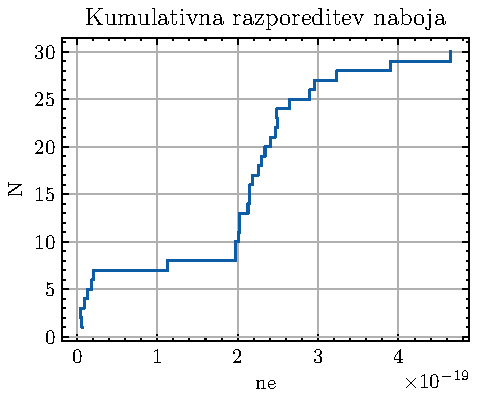
\includegraphics[width=13cm]{graf.pdf}
    \caption{Komulativen prikaz razporeditve naboja po kapljicah}
    \label{graf}
\end{center}
\end{figure}



\end{document}